
\section{Formularsysteme}

    Im folgenden Teil wird eine umfassende Analyse der derzeit führenden Methoden zur Implementierung von Formularen und Formularvalidierung durchgeführt. Dies zielt darauf ab, einen detaillierten Überblick über die aktuellen Best Practices und technologischen Ansätze zu bekommen.\cite{prompt10_pollak}

    \subsection{Wichtige Konzepte in \gls{react}}
    Bevor wir in die spezifischen Frameworks und Bibliotheken eintauchen, ist es wichtig, einige grundlegende Konzepte der Formularerstellung in React zu verstehen. Diese Konzepte bilden die Grundlage für viele der vorgestellten Frameworks und deren Architektur.
    
        \subsubsection{React Hooks\label{sec:ReactHooks}}
        Wie in der React-Dokumentation \cite{reacthooks} nachzulesen, sind React Hooks Funktionen, mit denen React-Features direkt in den Komponenten genutzt werden können. Sie erlauben es zum Beispiel, State und andere React-Features zu verwenden, ohne eine Klasse schreiben zu müssen. Ein State-Hook könnte beispielsweise folgendermaßen aussehen:
    
        \begin{lstlisting}[language=JavaScript]
    function Counter() { 
        const [count, setCount] = useState(0); 
        return (
            <div>
                <p>Count: {count}</p> 
                <button onClick={() => setCount(count + 1)}>Increment</button>  
            </div>
        );
    }
        \end{lstlisting}
        In diesem Beispiel wird count durch den ''useState''-Hook verwaltet und durch die ''setCount''-Funktion aktualisiert.

        \subsubsection{Controlled und Uncontrolled Komponenten}
        Bei der Arbeit mit Formularen in \gls{react} gibt es zwei grundlegende Arten von Komponenten: Controlled- und Uncontrolled-Komponenten.
        
        \paragraph{Controlled Komponenten}
        Wie man in der React-Dokumentation \cite{react_forms} nachlesen kann, wird der Zustand bei Controlled Komponenten durch den React State verwaltet. Das bedeutet, dass jedes Eingabefeld seinen Wert aus dem State bezieht und jede Änderung des Werts den State aktualisiert. Controlled Komponenten bieten somit die vollständige Kontrolle über das Formular und die Eingabewerte.
        
        Abbildung \ref{fig:controlled-component} veranschaulicht den Datenfluss einer Controlled-Komponente. Jede Benutzereingabe löst ein Event aus, das vom Event-Handler verarbeitet wird, welcher wiederum den State aktualisiert. Der State gibt den neuen Wert an das Eingabefeld zurück, wodurch der Datenfluss vollständig kontrolliert wird.
        
        \begin{figure}[H]
            \centering
            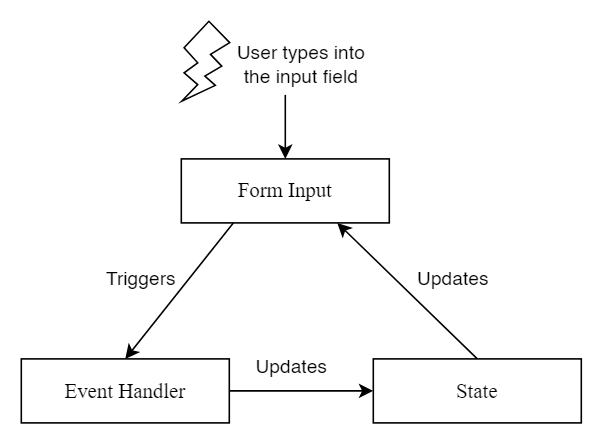
\includegraphics[width=0.7\linewidth]{images/controlledComponent.png}
            \caption{Datenfluss in Controlled Komponenten, Quelle: \cite{controlled_inputs_diagram}}
            \label{fig:controlled-component}
        \end{figure}

        Ein Beispiel für die Initialisierung des States und das Handling von Änderungen sieht wie folgt aus:
        
        \begin{lstlisting}[language=JavaScript]
        const [name, setName] = useState(""); 
        
        const handleChange = (e) => {
            setName(e.target.value); 
        };
        \end{lstlisting}
        
        In diesem Code wird der State für das Eingabefeld ''name'' initialisiert und mit der Funktion ''handleChange'' aktualisiert, sobald der Benutzer eine Eingabe tätigt. Jede Änderung des Eingabefelds löst ein Event aus, das vom Event-Handler verarbeitet wird, um den neuen Wert im State zu speichern.
        
        Die Verbindung zwischen dem State und dem Eingabefeld wird durch die Verwendung des Attributs ''value'' hergestellt.
        
        \begin{lstlisting}[language=JavaScript]
        return (
            <form onSubmit={handleSubmit}> 
                <input type="text" value={name} onChange={handleChange} />  
                <button type="submit">Submit</button> 
            </form>
        );
        \end{lstlisting}

        In diesem Beispiel wird der Wert des Eingabefeldes ''name'' durch den State gesteuert, und jede Änderung wird durch die Funktion ''handleChange'' verarbeitet.
        
        \paragraph{Uncontrolled Komponenten\label{sec:uncontrolledComponents}}
        Im Gegensatz zu Controlled Komponenten, wie in \cite{react_uncontrolled_components} beschrieben, wird bei Uncontrolled Komponenten der Zustand des Eingabefeldes nicht durch den React State, sondern direkt durch das DOM verwaltet. Dies bedeutet, dass der Wert eines Eingabefeldes über ein ''ref''-Objekt zugänglich ist, wodurch eine direkte Interaktion mit dem DOM ermöglicht wird.
        
        Ein Beispiel für die Initialisierung eines ''ref''-Objekts und dessen Verwendung sieht wie folgt aus:
        
        \begin{lstlisting}[language=JavaScript]
        const inputRef = useRef(); 
        
        const handleSubmit = (e) => {
            console.log(inputRef.current.value);  
        };
        \end{lstlisting}
        
        In diesem Code wird das ''ref''-Objekt durch die Funktion ''useRef'' initialisiert. Dieses Objekt ermöglicht den Zugriff auf das DOM-Element des Eingabefeldes. Die Funktion `handleSubmit` zeigt, wie der aktuelle Wert des Eingabefeldes über das ''ref''-Objekt abgerufen werden kann. Dies unterscheidet sich grundlegend von Controlled-Komponenten, bei denen der Wert im React-State gespeichert wird.
        
        Die vollständige Implementierung einer Uncontrolled-Komponente könnte wie folgt aussehen:
        
        \begin{lstlisting}[language=JavaScript]
        return (
            <form onSubmit={handleSubmit}> 
                <input type="text" ref={inputRef} />  
                <button type="submit">Submit</button>  
            </form>
        );
        \end{lstlisting}
        
        In diesem Beispiel verwenden wir ''useRef'' zur direkten Referenzierung des DOM-Elements und zum Abrufen des Werts, ohne den State von \gls{react} zu nutzen.
        
    \subsection{React Hook Form}
        \subsubsection{Funktionsweise und Architektur} 
        Wie in \cite{reacthookform} ausführlich beschrieben, ist React Hook Form ein leichtgewichtiges Framework, welches das einfache Implementieren von Formularen mit integrierter Validierung in \gls{react}-Anwendungen ermöglicht. Das Ziel dieses Frameworks ist die Optimierung der Benutzer- und Entwickler-Experience. Dies geschieht in erster Linie durch Performance-Optimierungen. Es basiert, wie der Name schon sagt, auf dem Prinzip der oben erklärten React Hooks \ref{sec:ReactHooks}. \cite{prompt12_pollak}

            \paragraph{Verwaltung von Formularzuständen}
            Das React Hook Form nutzt Uncontrolled Komponenten (siehe Abschnitt \ref{sec:uncontrolledComponents}), da der Formularzustand direkt im DOM verwaltet wird und nicht im React-State. Diese Architektur führt zu einer verbesserten Effizienz, da Re-Renders minimiert werden und die Performance dadurch gesteigert wird.

            \paragraph{Beispiel}
            Die Verwendung von React Hook Form beginnt mit der Initialisierung des Formulars und der Registrierung der Eingabefelder:
            
            \begin{lstlisting}[language=JavaScript]
            const { register, handleSubmit } = useForm(); 
            
            const onSubmit = (data) => {  
                console.log(data); 
            };
            \end{lstlisting}
            
            In diesem Codeblock wird das Formular initialisiert, indem der Hook ''useForm'' verwendet wird. Die Funktion ''register'' dient dazu, Eingabefelder mit dem Formular zu verbinden, während ''handleSubmit'' die Verarbeitung der Formulardaten beim Absenden übernimmt. Die Funktion ''onSubmit'' wird aufgerufen, um die eingegebenen Daten weiterzuverarbeiten.
            
            Im nächsten Schritt wird gezeigt, wie diese Funktionen in einem Formular integriert werden:
            
            \begin{lstlisting}[language=JavaScript]
        return (
            <form onSubmit={handleSubmit(onSubmit)}>  
                <input {...register("name")} placeholder="Name" />  
                <input {...register("age")} type="number" placeholder="Age" /> 
                <button type="submit">Submit</button>  
            </form>
        );
            \end{lstlisting}
            
            In diesem Beispiel werden zwei Eingabefelder (''name'' und ''age'') registriert. Durch die Verwendung des Spread-Operators (''...register'') werden die Felder direkt mit dem Formular verbunden. Beim Absenden des Formulars ruft der Button die Funktion ''handleSubmit'' auf, welche wiederum die Funktion ''onSubmit'' ausführt. Dies ermöglicht eine einfache Verwaltung und Verarbeitung der Formulardaten.

        \subsubsection{Performance \label{sec:perfomanceHookForm}}
        Wie oben schon erwähnt wurde, ist das Hauptziel dieses Frameworks die Optimierung der Performance. Dies geschieht durch das Minimieren der Re-Renders. 

        Re-Rendern ist der Prozess, bei dem Komponenten neu geladen werden müssen, um Änderungen im Zustand oder in den Properties widerzuspiegeln. Dies benötigt logischerweise Rechenleistung. Um dies zu optimieren, wird versucht, diese auf das Minimum zu reduzieren. Dafür sorgt im Wesentlichen folgende Strategie:\cite{prompt12_pollak}

            \paragraph{Isolierte Re-Renders und Subscriptions}
            Wenn ein Benutzer in ein Eingabefeld tippt, wird nur dieses spezifische Feld aktualisiert, ohne dass der gesamte Formularbaum neu gerendert wird. Isolierte Re-Renders konzentrieren sich darauf, den Bereich des Re-Renderings auf spezifische Teile einer Komponente zu beschränken. Subscriptions hingegen überwachen Änderungen bestimmter Werte und lösen Re-Renders nur für die betroffenen Komponenten aus. Jedoch ist anzumerken, dass Formik im Vergleich zu React Hook Form tendenziell mehr Re-Renders verursachen kann, insbesondere bei großen Formularen. \cite{prompt13_pollak} \cite{prompt14_pollak}
                
        \subsubsection{Integration anderer Validierungsbibliotheken}
        \label{sec:IntegrationReactHookForm}
        React Hook Form ermöglicht es auch, Validierungsschemata anderer Validierungsbibliotheken zu verwenden. Es können Yup, Zod, Superstruct und Joi verwendet werden. Dabei übernimmt die externe Bibliothek die Prüfung der Formulardaten, während React Hook Form die Verwaltung der Eingabefelder und Fehlernachrichten übernimmt. \cite{prompt11_pollak}
        
    \subsection{Formik}
       \subsubsection{Funktionsweise und Architektur} 
        Wie in \cite{formik} beschrieben, ist Formik ebenso ein weit verbreitetes Framework zur Erstellung von Formularen in React-Anwendungen. Diese Bibliothek zielt darauf ab, ein skalierbares und performantes Hilfstool für Formulare bereitzustellen, das mit einer minimalen API die besonders mühsamen Aufgaben übernimmt.
        
        \paragraph{Beispiel}
        Die Verwendung von Formik beginnt mit der Definition des Formulars und der Initialisierung der Werte. Ein einfaches Beispiel zeigt, wie die Komponente ''<Formik>'' verwendet wird, um ein Formular zu erstellen:
        
        \begin{lstlisting}[language=JavaScript]
        <Formik
            initialValues={{ name: "", age: "" }} 
            onSubmit={(values) => {  
                console.log(values); 
            }}
        >
        \end{lstlisting}
        
        Die Eigenschaften ''initialValues'' setzen die Startwerte für die Formularfelder, während ''onSubmit'' eine Funktion definiert, die beim Absenden des Formulars ausgeführt wird. Innerhalb dieser Funktion können die eingegebenen Werte verarbeitet werden.
        
        Der nächste Schritt besteht darin, die Formularfelder und den Absende-Button zu definieren. Dies wird mit der Komponente ''<Form>'' und ''<Field>'' realisiert, wie im folgenden Codeblock dargestellt:
        
        \begin{lstlisting}[language=JavaScript]
        {() => (
            <Form>  
                <Field name="name" placeholder="Name" />  
                <Field name="age" type="number" placeholder="Age" /> 
                <button type="submit">Submit</button>  
            </Form>
        )}
        </Formik>
        \end{lstlisting}

        \subsubsection{Performance}
        Formik legt großen Wert auf eine effiziente Handhabung von Formularen, indem es eine optimierte Zustandsverwaltung und Methoden zur Minimierung von Re-Renders bereitstellt. Das Optimieren des Re-Renderns erledigt Formik intern mittels React-Methoden. 
        Durch den oben erwähnten zentral geregelten Formularzustand kann durch die klare Trennung ebenso die Performance optimiert werden.
    
        \subsubsection{Integration anderer Validierungsbibliotheken}
        Formik unterstützt die Integration externer Validierungsbibliotheken wie Yup, Zod und Joi, um Validierungsregeln zu definieren. Dies funktioniert nach dem gleichen Prinzip wie bei React Hook Form \ref{sec:IntegrationReactHookForm}. \cite{prompt15_pollak}
    
    \subsection{React Final Form}
        \subsubsection{Funktionsweise und Architektur} 
        React Final Form\cite{reactfinalform} ist ein leichtgewichtiges und sehr flexibles Framework zur Erstellung von Formularen in React-Anwendungen. Es basiert auf einem Subscriptions-Based-Modell, bei dem Komponenten gezielt auf bestimmte Zustandsänderungen reagieren können, was zu einer performanteren Anwendung führt.
    
            \paragraph{Beispiel}
            Die Verwendung von React Final Form beginnt mit der Definition des Formulars und der zugehörigen ''onSubmit''-Funktion. Hier ein Beispiel, wie man das ''Form''-Element initialisiert und die Funktion definiert, die beim Absenden des Formulars aufgerufen wird:
            
            \begin{lstlisting}[language=JavaScript]
            const onSubmit = (values) => {  
                console.log(values); 
            };
            
            return (
                <Form
                    onSubmit={onSubmit}  
                    render={({ handleSubmit }) => (  
            \end{lstlisting}
            
             Die ''render''-Prop wird verwendet, um auf die ''handleSubmit''-Funktion zuzugreifen, die von React Final Form bereitgestellt wird.
            
            Im nächsten Schritt werden die Formularfelder und der Submit-Button innerhalb des ''render''-Props hinzugefügt:
            
            \begin{lstlisting}[language=JavaScript]
    <form onSubmit={handleSubmit}> 
        <Field name="name" component="input" placeholder="Name" />  
        <Field name="age" component="input" type="number" placeholder="Age" />  
        <button type="submit">Submit</button>  
    </form>
            \end{lstlisting}
            
            Dieser Code zeigt, wie die ''<Field>''-Komponente von React Final Form verwendet wird, um die Eingabefelder zu erstellen. Jedes ''<Field>''-Element ist mit einem Namen (''name'') versehen und verwendet die ''component''-Prop, um anzugeben, welches HTML-Element verwendet werden soll (in diesem Fall ''input'').
    
        \subsubsection{Performance}
        React Final Form legt besonderen Wert auf eine effiziente Performance. Durch das abonnementsbasierte Modell werden unnötige Re-Renderings vermieden, da nur die betroffenen Felder oder Komponenten aktualisiert werden. 
    
        \subsubsection{Validierung und Flexibilität}
        React Final Form bietet eine flexible Validierungslogik, die sowohl synchron als auch asynchron unterstützt. Validierungen können für einzelne Felder oder für das gesamte Formular definiert werden. \cite{prompt16_pollak}


    \subsection{Zod}
        \subsubsection{Funktionsweise und Architektur} 
        Wie in der Dokumentation nachzulesen ist, ist Zod\cite{zod} im Gegensatz zu den zuvor erwähnten Frameworks kein Formularmanagement-Tool, sondern eine moderne und minimalistische Validierungsbibliothek, die für TypeScript geeignet ist. Zod ist eher komplementär zu React Hook Form und Formik. Sie ist besonders für TypeScript-Anwendungen geeignet, da sie nicht nur Daten validiert, sondern gleichzeitig auch die Typen (also die Struktur und Art der Daten, z. B. Zahlen oder Texte) automatisch für TypeScript ableitet. 

        \subsubsection{Performance}
        Zod ist leichtgewichtig, was bedeutet, dass es nicht viel Speicher und Rechenleistung benötigt. Daher erfolgt die Validierung schnell, auch bei komplexeren Validierungen. Die Performance wird ebenso dadurch optimiert, dass es keine Abhängigkeiten von anderen Bibliotheken hat. Es ist ein sogenanntes Standalone-Framework.

        \subsubsection{Flexibilität und Validierungsmöglichkeiten}
        Zod bietet eine enorme Flexibilität, um komplexe Regeln zu definieren. Beispielsweise könnten Mindest- oder Höchstwerte, Pflichtfelder oder auch benutzerdefinierte Validierungen durchgeführt werden. Eine benutzerdefinierte Regel könnte folgend aussehen:

        \begin{lstlisting}[language=JavaScript]
        const schema = z.string().refine((val) => val.startsWith("A"), {  
            message: "Der Wert muss mit 'A' beginnen",
        });
        \end{lstlisting}
        
        Dieser Code definiert ein Zod-Schema, das überprüft, ob ein gegebener Wert ein String ist und mit dem Buchstaben ''A'' beginnt. Die Methode ''.refine()'' wird verwendet, um eine benutzerdefinierte Validierungsregel hinzuzufügen.
        
        Nachdem das Schema definiert wurde, kann es verwendet werden, um Werte zu überprüfen und festzustellen, ob sie gültig sind. Hier ein Beispiel, wie das Schema verwendet werden kann, um Werte zu validieren:
        
        \begin{lstlisting}[language=JavaScript]
        const result = schema.safeParse("Alice");  
        const result2 = schema.safeParse("Bob"); 
        \end{lstlisting}
        
        In diesem Beispiel wird die Methode ''.safeParse()'' verwendet, um die Werte ''Alice'' und ''Bob'' anhand des Schemas zu überprüfen. Diese gibt ein Objekt zurück, das angibt, ob die Validierung erfolgreich war oder nicht. Im Falle von ''Alice'' ist die Validierung erfolgreich, da der Wert mit ''A'' beginnt. Im Falle von ''Bob'' schlägt die Validierung fehl, da der Wert nicht mit ''A'' beginnt.
